\documentclass[11pt]{article}
\usepackage[utf8]{inputenc}
\usepackage{graphicx}
\graphicspath{ {images/} }
\usepackage{amsmath}
\usepackage{placeins}

\title{Coursework 1 – Transient Conduction}
\author{Adam Duncan}
\date{\today}

\begin{document}

\maketitle

\section{\emph{Part A: Using lumped capacitance}}
\subsection{Assumptions}
\begin{itemize}
	\item Internal temperature of the steel ball is uniform at any time t.
	\item No change in water temperature
	\item No heat transfer by radiation
	\item Material is standard carbon steel
	\item Material properties constant (taken at average temperature $T = 469 ^{o}C$)
\end{itemize}
\subsection{Properties}
\begin{table}[h]
	\centering
	\caption{Properties from problem}
	\begin{tabular}{lllll}
		Property & Value & Unit &  &  \\ \cline{1-3}
		Characteristic   length, L & 5 & cm &  &  \\
		Diameter, D & 10 & cm &  &  \\
		Temperature   of the water, $T_w$ & 38 & $^oC$ &  &  \\
		Initial   temperature of steel ball, $T_{s,1}$ & 900 & $^oC$ &  &  \\
		Final   temperature of steel ball, $T_{s,2}$ & 200 & $^oC$ &  &  \\
		Heat transfer   coefficient, h & 600 & $W/m^{2}K$ &  & 
	\end{tabular}
	\label{tab1}
\end{table}

\begin{table}[h]
	\centering
	\caption{Properties from literature}
	\begin{tabular}{llll}
		Property & Value at $T_{avg}$(469 $^{o}C$) & Unit & Source \\ \hline
		Specific heat   capacity, Cp & 552 & $J\cdot kg^{-1} K^{-1}$ & \cite{jean-marc_franssen_fire_2015} \\
		Density & 7.8 x $10^3$ & $kg\cdot m^{-3}$ & \cite{bergman_fundamentals_2011} \\
		Conductivity & 40 & $W\cdot m^{-1} K^{-1} $& \cite{jean-marc_franssen_fire_2015}
	\end{tabular}
	\label{tab2}
\end{table}
\FloatBarrier

The density of steel is assumed to be constant over the temperature range so the value in table \ref{tab2}, which is given at 300K, is assumed to be accurate. To confirm this assumption is acceptable the elongation was calculated using the ISO 834 standard equations\cite{jean-marc_franssen_fire_2015}. This showed the overall change in volume of the sphere was ~3\% over the full temperature range of the problem. As $V \propto \rho$ this change is low enough to be discounted and for the assumption to be justified.

\subsection{Schematic}
\begin{figure}[!htbp]
	\centering
	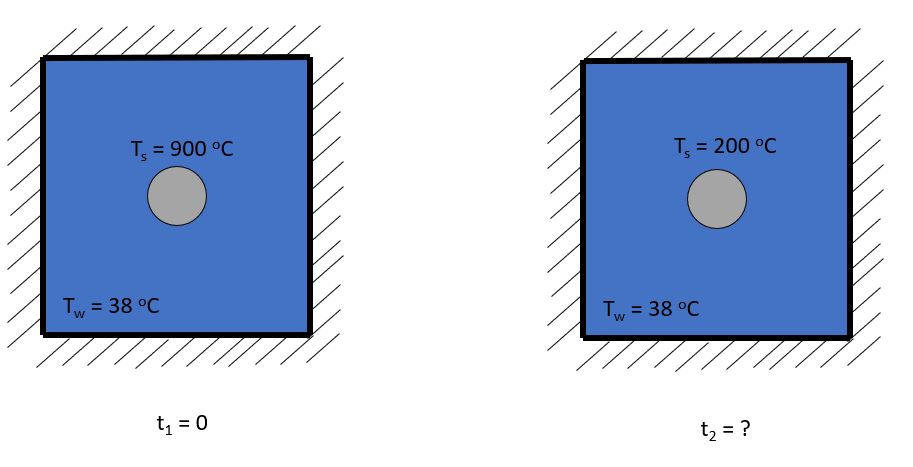
\includegraphics[width=0.85\textwidth]{part_a_fig}
	\caption{Part A schematic at initial and final state.}
	\label{fig:schem_a}
\end{figure}
\FloatBarrier
\subsection{Analysis}

Energy balance for closed system gives the following equation.
\begin{equation}\label{eqn_1}
	\stackrel{.}{Q} = hA(T_{s}-T_{f}) = C_{p}\rho V \frac{dT_{c}}{dt}
\end{equation}

Where $\stackrel{.}{Q}$ is heat [$W$], $h$ is the heat transfer coefficient [$W/m^{2}K$], $A$ is the surface area between the ball and water [$m^{2}$], $T_{s}$ is the temperature of the steel ball [$^{o}C$], $T_{f}$ is the temperature of the water [$^{o}C$], $C_{p}$ is the specific heat capacity [$J/mK$], $\rho$ is the density of the steel ball[$kg/m^{3}$], $V$ is the volume of the steel ball [$m^3$] and $t$ is the time [$s$].
\newline

Rearranging (\ref{eqn_1}) to separate the variables gives.
\begin{equation}\label{key}
	\frac{1}{T_{s}-T_{f}} dT_{c} = \frac{hA}{C_{p}\rho V}dt
\end{equation}

Which integrates to give.
\begin{equation}\label{eqn_3}
	\ln{(\frac{T_{s1}-T_{f}}{T_{s2}-T_{f}})} =  \frac{hA}{C_{p}\rho V}(t_{2}-t_{1})
\end{equation}
Where $t_{i}$ and $T_{si}$ are the time [s] and temperature [$^oC$] receptively at state i.

Rearranging (\ref{eqn_3}) to make $t_{2}$ the subject gives.
\begin{equation}\label{key}
	t_{2} = \frac{C_{p}\rho V}{hA}(\ln{(\frac{T_{s1}-T_{f}}{T_{s2}-T_{f}})})
\end{equation}

Substituting in the values for the variables given in Figure \ref{fig:schem_a} gives the final value.
\boldmath
\begin{equation}\label{key}
	t_2 = 205 s
\end{equation}
\unboldmath
Where $t_2$ is the time for the steel ball to reach a temperature of $200^{o}C$ under given assumptions.

\section{\emph{Part B: Lumped capacitance justification}}
The lumped capacitance method is only valid if the ratio of the conductive heat transfer to convective heat transfer is low. This ratio is known as the Biot number, $Bi$, and is given by.
\begin{equation}\label{eqn_biot}
	Bi = \frac{h \cdot L_{c}}{k}
\end{equation}
Where $h$ is convective coefficient [$W/m^{2}K$], $L_{c}$ is the characteristic length [m] and $k$ is the conductivity [$W/m \cdot K$]. 

Applying the values from Tables \ref{tab1} and \ref{tab2}, choosing to set $L_{c}=R$ and substituting into equation \ref{eqn_biot} gives:
\begin{equation}\label{key}
	Bi = 0.7
\end{equation}

If $Bi > 0.1$ then the lumped capacitance method is no longer applicable as the assumptions made introduce non-trivial errors \cite{bergman_fundamentals_2011}. This means that the result in part A likely inaccurate.

It is worth noting however that the choice of $L_c$ is significant. it is common to select $L_c$ to be the maximum distance over which a temperature gradient would occur, as has been done above, but the method from the mathematical derivation is to use $L_c = \frac{V}{A_s}$ which for a sphere gives $L_c = \frac{R}{3}$. This means the use of $L_c = R$ will tend to overestimate the value of $Bi$. In this case however, using $L_c = \frac{R}{3}$ gives $Bi = 0.25$ so the result can still be assumed to be inaccurate despite the overestimate.

\section{\emph{Part C: Transient conduction}}
\begin{equation}
	t=\frac{f_{0} \rho C_{p} R^{2}}{k}
\end{equation}
\section{\emph{Part D: Non-infinite water bath}}

\section{\emph{Part E: Equilibrium temperature}}

\bibliographystyle{plain}
\bibliography{refs}
\end{document}

